%++++++++++++++++++++++++++++++++++++++++
% Don't modify this section unless you know what you're doing!
\documentclass[letterpaper,12pt]{article}
\setlength{\parindent}{4ex}
\setlength{\parskip}{1ex}

\usepackage{graphicx}
\usepackage{indentfirst}
\usepackage{tabularx} % extra features for tabular environment
\usepackage{subfigure} 

\usepackage{caption} % Spacing between caption (title) and actual table
\captionsetup[table]{skip=10pt}

\usepackage{amsmath}  % improve math presentation
\usepackage{graphicx} % takes care of graphic including machinery
\usepackage{pgfplots}
\usepackage[margin=1in,letterpaper]{geometry} % decreases margins
\usepackage{cite} % takes care of citations
\usepackage[final]{hyperref} % adds hyper links inside the generated pdf file
\hypersetup {
	colorlinks=true,       % false: boxed links; true: colored links
	linkcolor=blue,        % color of internal links
	citecolor=blue,        % color of links to bibliography
	filecolor=magenta,     % color of file links
	urlcolor=blue         
      }
      \setcounter{tocdepth}{3}

\usepackage{pgfplots}      


% ++++++++++++++++++++++++++++++++++++++++

\begin{document}

\title{CS 7641 Machine Learning \\
		\ Assignment 1 }
\author{David Yun}
\date{September 23, 2018}
\maketitle

\begin{abstract}
  The implementation, and basic fundamentals behind the following Machine Learning Algorithms will be discussed in detail:  
  \begin{enumerate}
    \item Decision trees with some form of pruning
    \item Neural Networks
    \item Boosting
    \item Support Vector Machines (SVM)
    \item k-Nearest Neighbors (kNN)
      
    \end{enumerate}

    For this assignment, Python is used, along with the necessary libraries associated within each topic.  The full code files are available on github\footnote{David Yun's Github: \url{https://github.com/tree-fiddy/Assignment_1}}
    Please refer to the README.txt file for concise instructions on how to run the files associated with each aforementioned algorithms.  The full README.md file will guide a reader on how to use the files to better understand the objectives of this Assignment.  

\end{abstract}

\tableofcontents

\section{Decision Trees: Setup Information}

The implementation of Decision Trees was borrowed from my previous coursework in CSE6242 (Data Visualization) with minor tweaks.
\textbf{Cross-Validation} is done without the need for a training-validation split here because of the use of Random Forests, which is a collection of decision trees.  Random forests allow us to create a robust model with less variance which results in a reduction in overfitting\footnote{By averaging several decision trees, the result is a less likely chance of overfitting}.  With proper pruning (Entropy thresholds \& Max Depth), one can further reduce the variance of the model and further decrease the chance of overfitting.  The \textbf{dataset} used is the UCI Credit Approval Dataset\footnote{UCI Credit Approval Data Set: \url{http://archive.ics.uci.edu/ml/datasets/credit+approval}}.  Some small adjustments were made to the dataset, such as removing rows where data was missing.  

\subsection{Learning Curves Analysis}
The accuracy of our decision tree relies on our tolerance for pre-pruning.  In essence, one must specify \emph{when} to stop growing the tree.  On one extreme, we can set a condition to stop growing the tree once we reach a \emph{pure\footnote{A leaf is said to be ``pure'' if the leaf contains homogenous labels.  By extension, this equates to a situation where Entropy equals 0.}} leaf.  However, this will likely make the tree longer than need be.  A more depth-restrictive approach is to set an arbitrary threshold for Entropy in our Decision Tree, where we will halt further node and leaf generation if the current node produces leaves with Entropy values less than our specified threshold.  To ensure the efficacy of our pre-pruning process, we also incorporate a limit to the depth of our tree to 5.  This will handle extreme cases where our dataset is so large, that splitting across many features is possible. This also has the added benefit of dramatic performance improvement, without sacrificing accuracy, when compared to not setting a depth and letting the tree grow indefinitely.  The performance of our decision tree, while varying \text{threshold levels} is highlighted in Table \ref{table:PrePruningTable}.

\begin{table}[htb]
  \caption{Pre-Pruning Spec Performance (forest size = 50)}
  \label{table:PrePruningTable}
  \centering
  \begin{tabular}{|c|c|c|}
  
    \hline
    \hline
    \multicolumn{1}{c}{Entropy Threshold}
    &  \multicolumn{1}{c}{Model Accuracy} \\
    \cline{1-2}
    0.0 & 0.86 \\
    \cline{1-2}
    0.1 & 0.86 \\
    \cline{1-2}
    0.2 & 0.60 \\
    \cline{1-2}
    0.3 & 0.57 \\
    \cline{1-2}
    0.4 & 0.55 \\
    \cline{1-2}
    0.5 & 0.55 \\
    \cline{1-2}
    0.6 & 0.54 \\
    \cline{1-2}
    0.7 & 0.54 \\
    
    
    \cline{1-2}
  \end{tabular}
\end{table}

\begin{figure}
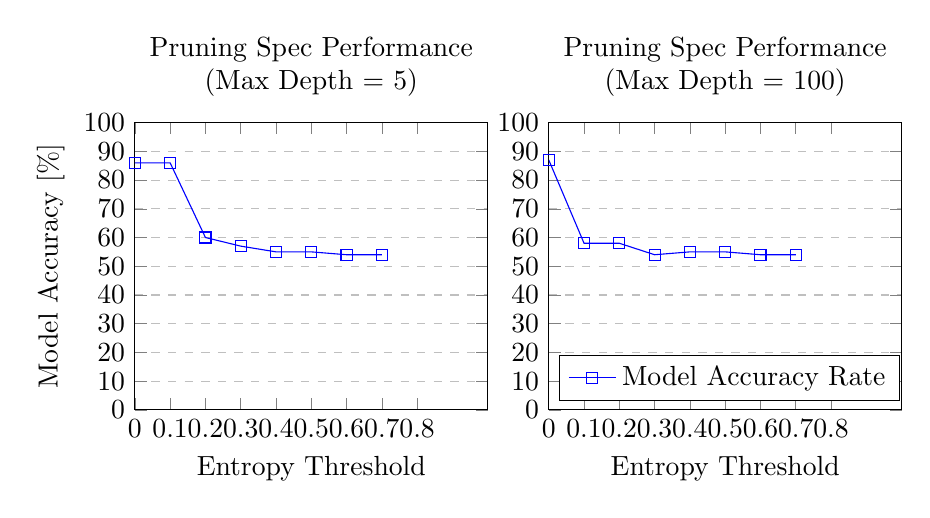
\begin{tikzpicture}[every axis/.append style={width=0.5\linewidth,title style={align=center}}]

  \begin{axis} [
    name = axis1,
    title = {Pruning Spec Performance \\ (Max Depth = 5)},
    xlabel = {Entropy Threshold},
    ylabel = {Model Accuracy [\%]},
    xmin = 0, xmax = 1,
    ymin = 0, ymax = 100,
    xtick={0,0.1,0.2,0.3,0.4,0.5,0.6,0.7,0.8},
    ytick={0,10,20,30,40,50,60,70,80,90,100},
    legend pos = south west,
    ymajorgrids=true,
    grid style = dashed
    ]
    \addplot[
    color = blue,
    mark = square,
    ]
    coordinates {
      (0.0,86)(0.1, 86)(0.2, 60)(0.3,57)(0.4,55)(0.5,55)(0.6,54)(0.7,54)
    };
  \end{axis}
  
  \begin{axis} [
    at={(axis1.outer north east)}, anchor=outer north west,
    name=axis2,
    title = {Pruning Spec Performance \\ (Max Depth = 100)},
    xlabel = {Entropy Threshold},
    %ylabel = {Model Accuracy [\%]},
    xmin = 0, xmax = 1,
    ymin = 0, ymax = 100,
    xtick={0,0.1,0.2,0.3,0.4,0.5,0.6,0.7,0.8},
    ytick={0,10,20,30,40,50,60,70,80,90,100},
    legend pos = south west,
    ymajorgrids=true,
    grid style = dashed
    ]
    \addplot[
    color = blue,
    mark = square,
    ]
    coordinates {
      (0.0,87)(0.1, 58)(0.2, 58)(0.3,54)(0.4,55)(0.5,55)(0.6,54)(0.7,54)
    };
    \legend{Model Accuracy Rate}
    
 
  \end{axis}
\end{tikzpicture}

\caption{Learning Curves} \label{fig:LearningCurves}
\end{figure}


As you can see, the model's accuracy reached an asymptote of around 50\% accuracy, which indicates that setting a higher threshold for Entropy renders this model's efficacy no better than a coin flip.  Thus, setting a pre-pruning specification is quite important here.  More notable is the fact that using the extreme case where Entropy must equal 0 before considering the tree complete yielded the same results as a 0.1 threshold.  However, computation times were slightly longer for this case, as more nodes had to be constructed until the threshold was met.  While in our dataset, it wasn't a huge factor, this is an important consideration one should make when building models on much larger data.  When the efficacy/accuracy of a model isn't compromised, any measures to speed up performance is a welcomed consideration.

You can also see that increasing the depth of the tree produced slightly better results \textbf{only} when we didn't set a threshold.  However, the computational time increased dramatically.  Moreover, setting entropy thresholds while allowing the tree to grow up to 100 levels deep caused this model to perform very poorly.

\section{Model Complexity Analysis}
Besides varying the Entropy Threshold \& Max Depth, we can also vary the \textbf{forest size} hyperparameter in our random forest.  Note here that we vary the hyperparameter, while holding the Entropy Threshold to 0.1 as supported by Figure \ref{fig:LearningCurves}.

\begin{figure}
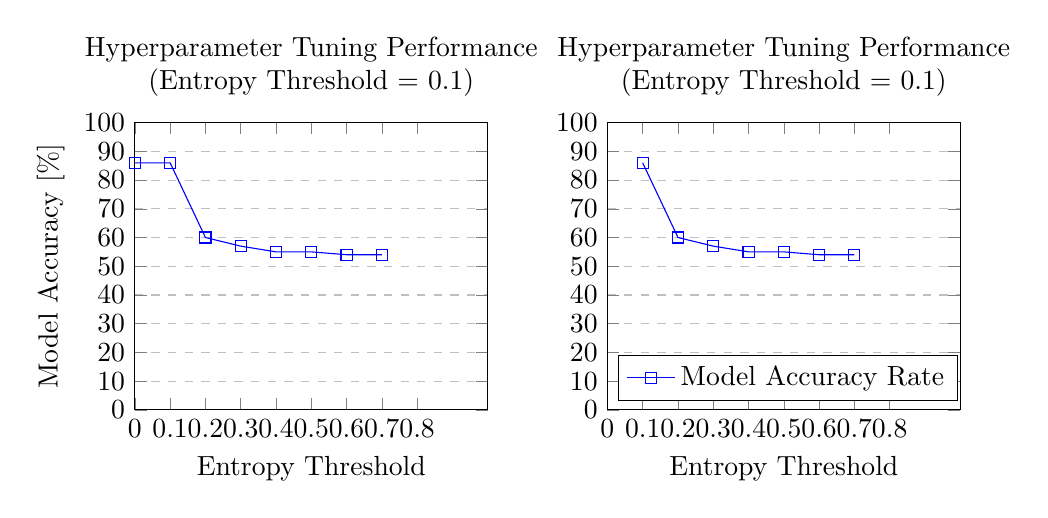
\begin{tikzpicture}[every axis/.append style={width=0.5\linewidth,title style={align=center}}]

  \begin{axis} [
    name = axis1,
    title = {Hyperparameter Tuning Performance \\ (Entropy Threshold = 0.1)},
    xlabel = {Entropy Threshold},
    ylabel = {Model Accuracy [\%]},
    xmin = 0, xmax = 1,
    ymin = 0, ymax = 100,
    xtick={0,0.1,0.2,0.3,0.4,0.5,0.6,0.7,0.8},
    ytick={0,10,20,30,40,50,60,70,80,90,100},
    legend pos = south west,
    ymajorgrids=true,
    grid style = dashed
    ]
    \addplot[
    color = blue,
    mark = square,
    ]
    coordinates {
      (0.0,86)(0.1, 86)(0.2, 60)(0.3,57)(0.4,55)(0.5,55)(0.6,54)(0.7,54)
    };
  \end{axis}
  
  \begin{axis} [
    at={(axis1.outer north east)}, anchor=outer north west,
    name=axis2,
    title = {Hyperparameter Tuning Performance \\ (Entropy Threshold = 0.1)},
    xlabel = {Entropy Threshold},
    %ylabel = {Model Accuracy [\%]},
    xmin = 0, xmax = 1,
    ymin = 0, ymax = 100,
    xtick={0,0.1,0.2,0.3,0.4,0.5,0.6,0.7,0.8},
    ytick={0,10,20,30,40,50,60,70,80,90,100},
    legend pos = south west,
    ymajorgrids=true,
    grid style = dashed
    ]
    \addplot[
    color = blue,
    mark = square,
    ]
    coordinates {
      (0.1,86)(0.1, 86)(0.2, 60)(0.3,57)(0.4,55)(0.5,55)(0.6,54)(0.7,54)
    };
    \legend{Model Accuracy Rate}
    
 
  \end{axis}
\end{tikzpicture}

\caption{Learning Curves} \label{fig:LearningCurves}
\end{figure}


\section{Artificial Neural Networks:  Setup Information}

\subsection{Learning Curves Analysis}
To get a basic understanding of how our model performed, we first start off with a ``basic'' neural net with the following specifications:  (1) 1 Hidden Layer of size 30.  (2) Activation Function = 'relu' (rectified linear unit function, returns f(x) = max(0,x)) (3) L2 Regularization Alpha = 0.  The figure in Figure \ref{fig:ANN Learning Curves} shows the results with the aforementioned specifications, but letting our L2 Regularization/Penalty term to vary from 0 \& 10.


\begin{figure} %
  \centering
  \subfigure[L2 Regularization = 0] {%
    \label{fig:ANN Learning Curve L2 = 0}%
    \includegraphics[height=2in]{Neural_Nets/output/ANN_Accuracy_Rates.png}}%
  \hspace{8pt}%
  \subfigure[L2 Regularization = 10]{%
    \label{fig:ANN Learning Curve L2 = 10}%
    \includegraphics[height=2in]{Neural_Nets/output/ANN_Accuracy_Rates2.png}}
  \caption{Learning Curves:  Testing vs. Training Sets w/ Varying Alpha (L2-Norm)}\label{fig:ANN Learning Curves}
\end{figure}

As you can see, specifying a larger L2 Penalty term reduces the accuracy of our both our Training and Test data.  While L2=0 produces a training set that is close to 100\% accuracy, the L2=10 rendition produces a training that is 86\% at it's best.     
\subsection{Model Complexity Analysis}
We can further optimize our analysis by letting other parameters in our Neural Network to vary.  For one, we can add complexity by increasing both the depth and size of our hidden layers.

\begin{figure} %
  \centering
  \subfigure[3 Hidden Layers, 30 Nodes Each] {%
    \label{fig:ANN Complexity Curve Layer30x3}%
    \includegraphics[height=2in]{Neural_Nets/output/ANN_Accuracy_Rates3.png}}%
  \hspace{8pt}%
  \subfigure[1 Hidden Layer, 28 Nodes]{%
    \label{fig:ANN Complexity Curve}%
    \includegraphics[height=2in]{Neural_Nets/output/ANN_Accuracy_Rates4.png}}
  \caption{Complexity Curves:  Testing vs. Training Sets w/ Varying Depth and Number of Hidden Layer Nodes}\label{fig:ANN Complexity Curves}
\end{figure}

The first figure in \ref{fig:ANN Complexity Curves} produces very promising results.  With 30 nodes in each of the 3 Hidden Layers, we achieve 100\% fit in the training set, and 86\% in the test set with only 32 weight-adjustment iterations (backpropogation).  However, one should be weary of these results, as it's highly suggestive of overfitting.  The speed in which the training accuracy improves is highly suggestive of this.  The right graph uses the $basicResults.best\_params\_$ method made available in scikitlearn to choose the best parameter for our ANN.  The best parameters are:  (1) L2 Penalty: 0.00316 (2) Hidden Layer Depth: 1 (3) Hidden Layer Size: 28 (4) Activation Function: Logistic.  Note that the figure on the right suggests we can reach a generalizable and accurate (88\% test accuracy rate with 99\% training accuracy rate) model with anywhere between 512-1024 weight-adjustment iterations.  
\end{document}
